\section{Overview}

\begin{frame}[c]{Learning Goals} 
    \large
    \begin{itemize}[<+(1)->]
        \item Gain familiarity with the transformer architecture and understand how it works
        \item Understand Tokens and Embeddings
        \item Comprehend how Attention works
        \item Become aware of common compression techniques
        \item Recognize limitations
    \end{itemize}
    \pause
    \textbf{Key Takeaway:} Transformers can be powerful, it might be worth
    trying to use them.
\end{frame}

\addtocounter{framenumber}{1}
\begin{frame}[standout]
    \huge
    Ask if you have questions \\
    or anything is unclear
    \pnote{
        I will be jumping around different topics a bunch \\
        Ask immediately if anything is unclear
    }
\end{frame}

\begin{frame}[c]{Overview}
    \begin{figure}
        \begin{columns}
            \column{0.8\linewidth}
            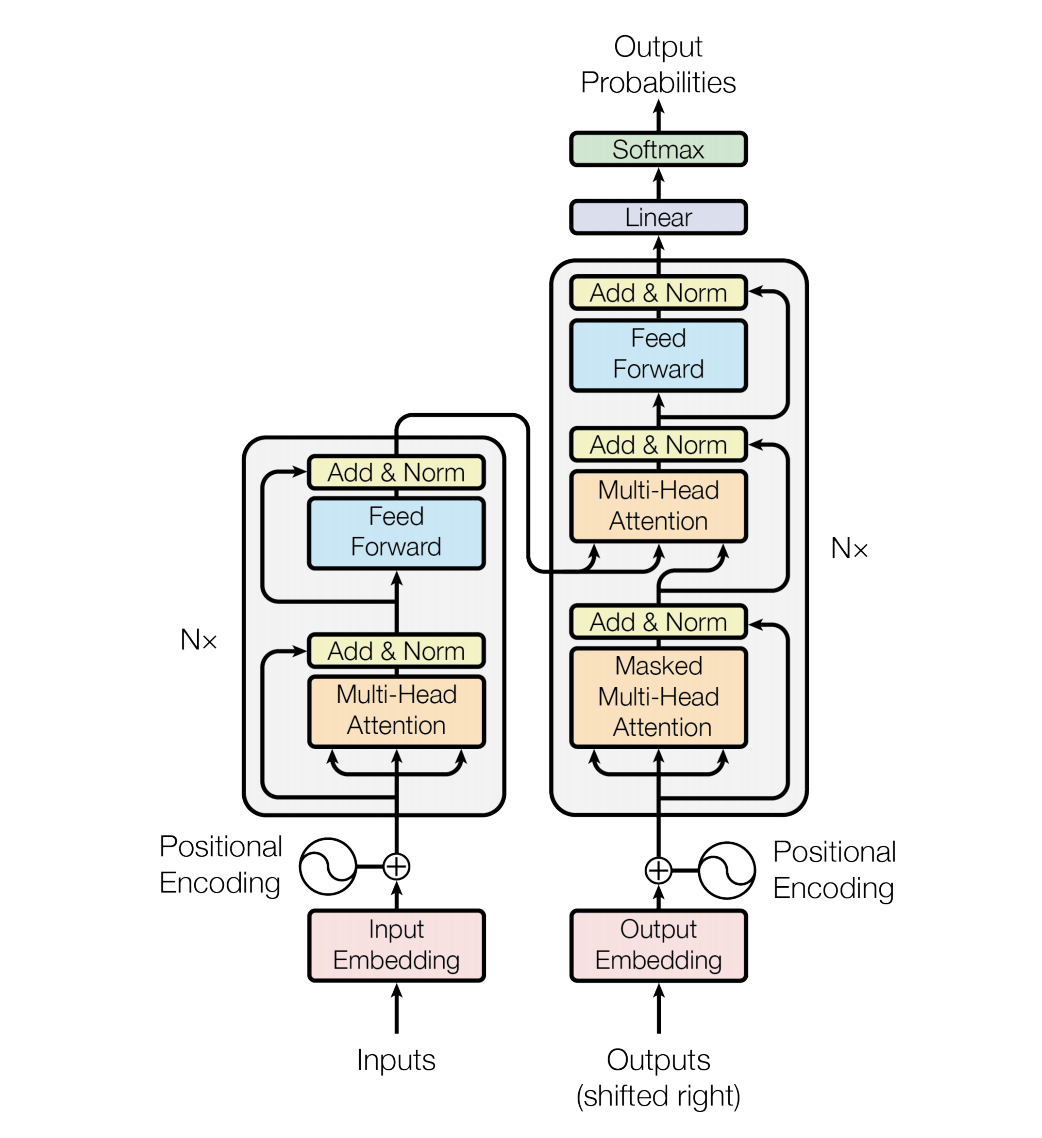
\includegraphics[height=0.9\textheight]{transformer}
            % \column{0.2\linewidth}
            \column{\dimexpr0.15\linewidth+9em}
            \raisebox{3em}{Image Source: \cite{vaswani_attention_2017}}
        \end{columns}
    \end{figure}
\end{frame}
